\documentclass[a4paper, 11pt]{article}


% -- Coments
\usepackage{verbatim}

% -- Fuente --
% \usepackage{fontspec}
% \setmonofont{JetBrainsMono Nerd Font}  

% -- Color --
\usepackage{xcolor}
%\definecolor{azul}{RGB}{00,33,99}
\definecolor{azul}{RGB}{35,72,180}

% -- Page Margin --
\usepackage[margin=1in]{geometry}

% -- Espaciados --
\newcommand{\Pspace}{0.5cm}
\newcommand{\Aspace}{0.2cm}

% -- Columnas --
\usepackage{multicol}

% -- Imagenes --
\usepackage{graphicx}
\usepackage{float}

% -- Matemáticas --
\usepackage{amsmath, amssymb}

% -- Gráficas --
\usepackage{pgfplots}
\pgfplotsset{compat=1.18}

% -- Código --
% \usepackage{minted}

\usepackage{minted}
\setminted{
    fontsize=\small,
    breaklines=true,               % Ajusta el código al ancho de página
    frame=lines,                   % Añade líneas arriba y abajo
    framesep=2mm,
    baselinestretch=1.2,
    bgcolor=lightgray!10           % Color de fondo muy suave
}
\newcommand{\mips}[1]{\mintinline{mips}{#1}}
\newcommand{\asm}[1]{\mintinline{asm}{#1}}
\newcommand{\clang}[1]{\mintinline{c}{#1}}
\newcommand{\az}[1]{{\color{azul}{#1}}}

\usepackage{listings}
\lstset{
    language=C,                     % Lenguaje del código
    basicstyle=\ttfamily\small,     % Fuente del código
    keywordstyle=\color{blue},      % Color de palabras clave
    commentstyle=\color{gray},      % Color de comentarios
    stringstyle=\color{red},        % Color de cadenas
    numbers=left,                   % Números de línea a la izquierda
    numberstyle=\tiny\color{gray},
    breaklines=true,                % Permitir saltos de línea
    frame=single                    % Marco alrededor del código
}

\usepackage[colorlinks=true, linkcolor=blue, urlcolor=blue]{hyperref}

\begin{comment}
-- Formato de pregunta simple
    % - Problema n
    \vspace{\Pspace}
    \item Problema \par
        % Respuesta:
        \vspace{\Aspace} \par
        { \color{azul}  }


 -- Formato de pregunta multimple
    % - Problema 
    \vspace{\Pspace}
    \item  \par
        % Respuestas:
        \vspace{\Aspace} \par
        a) 
        \\ { \color{azul} }

        \vspace{\Aspace} \par
        b) 
        \\ { \color{azul} }

        \vspace{\Aspace} \par
        c) 
        \\ { \color{azul} }


 -- Formato de imagen
\begin{figure}[!ht]
    \centering
    \includegraphics[width=0.5\textwidth]{}
\end{figure}


 -- Formato de tabla
\begin{tabular}{c|c}
    \textbf{A} & \textbf{B} \\
    \hline
    Texto & Texto \\
    Texto & Texto
\end{tabular} \\
\end{comment}


\title
{
    Arquitectura de Computadoras 2026-1 \\
    Tarea 3
}

\begin{document}

\maketitle

\begin{center}
    \begin{tabular}{r|l}
        \textbf{Expediente} & \textbf{Nombre} \\ \hline
        223210350 & Amaya Soria Angel Alberto \\
        219208106 & Bórquez Guerrero Angel Fernando \\
        223215039 & Miranda Sánchez Javier Leonardo \\
        223203899 & Tostado Cortes Dante Alejandro
    \end{tabular}
\end{center}

\rule{\linewidth}{0.3mm}

\vspace{0.3cm}
\begin{enumerate}
% - Problema 1
\vspace{\Pspace}
\item Suponer una CPU superescalar con scheduling dinámico con las siguientes características: \par
\begin{itemize}
    \item Emisión: 1 instrucción por ciclo.
    \item Compromiso: 1 instrucción por ciclo.
    \item ROB con suficientes entradas.
    \item Estaciones de reserva suficientes.
    \item Latencias: lw (2 ciclos), add (2 ciclos), mul (4 ciclos).
\end{itemize}
Usando el algoritmo de Tomasulo, simular la ejecución del siguiente programa y llenar la tabla: \\
\begin{figure}[!ht]
\centering
\begin{tabular}{|l|c|c|c|c|}
    \hline
    \textbf{Instrucción} & \textbf{Emisión} & \textbf{Ejecución} & \textbf{Escritura} & \textbf{Compromiso} \\
    \hline
    \mips{lw f2, 0(r1)} & \az{} & \az{} & \az{} & \az{} \\
    \hline
    \mips{lw f4, 0(r2)} & \az{} & \az{} & \az{} & \az{} \\
    \hline
    \mips{mul f6, f2, f4} & \az{} & \az{} & \az{} & \az{} \\
    \hline
    \mips{add f2, f6, f4} & \az{} & \az{} & \az{} & \az{} \\
    \hline
    \mips{add f8, f2, f4} & \az{} & \az{} & \az{} & \az{} \\
    \hline
    \mips{mul f10, f8, f2} & \az{} & \az{} & \az{} & \az{} \\
    \hline
    \mips{add f6, f2, f8} & \az{} & \az{} & \az{} & \az{} \\
    \hline
    \mips{add f12, f6, f10} & \az{} & \az{} & \az{} & \az{} \\
    \hline
\end{tabular}
\end{figure}



\newpage
% - Problema 2
\vspace{\Pspace}
\item La figura 5.44 (página 472 del libro Computer Organization and Design) \par indica que la política de escritura (write policy) del caché primario (L1) de ARM Cortex-A8 es "write-back, write-allocate". Investigar esta política y describirla brevemente. \\
\renewcommand{\thefigure}{5.\arabic{figure}}
\setcounter{figure}{43}
\begin{figure}[!ht]
    \centering
    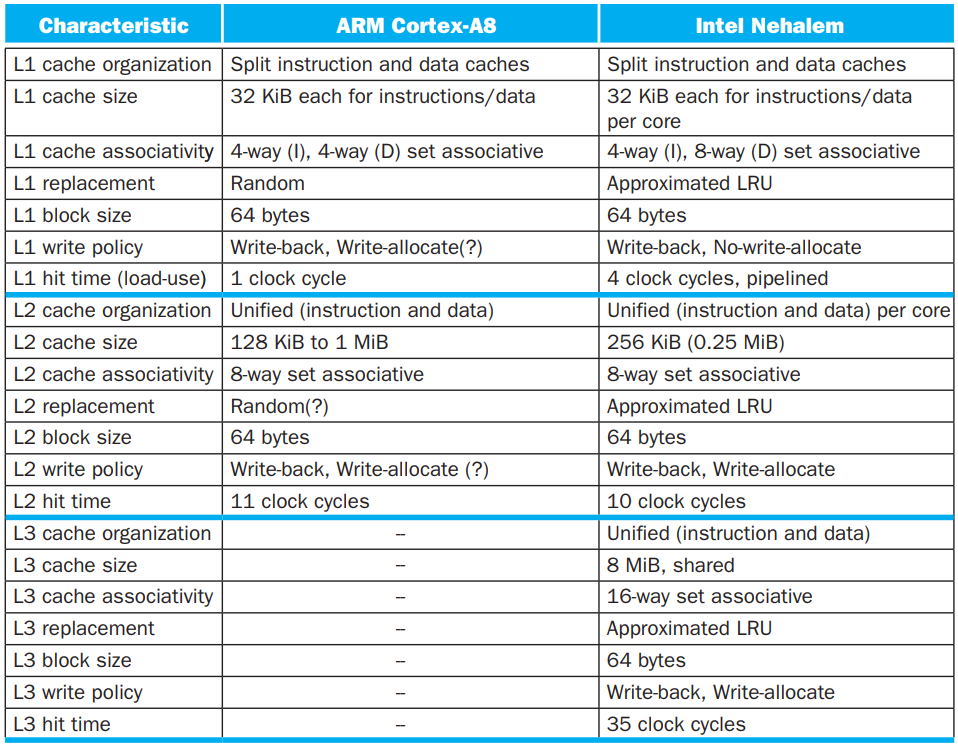
\includegraphics[width=0.8\textwidth]{./img/figure_5.44.png}
    \caption{Caches in the ARM Cortex-A8 and Intel Core i7 920.}
\end{figure}
\renewcommand{\thefigure}{\arabic{figure}} % restore default afterward
    % Respuesta:
    \vspace{\Aspace} \par
    { \color{azul}  
        \textbf{write-back} \par
        Cuando el procesador escribe un dato, la modificación se realiza únicamente en el caché. 
        El bloque modificado se marca con un dirty bit. 
        La escritura de memoria principal ocurre solo cuando el bloque es desalojado del caché. 
        Esto reduce el tráfico al bus de memoria comparado con \textbf{write-through}, 
        ya que múltiples escrituras al mismo bloque generan una sola escritura a memoria. \\

        \textbf{write-allocate} \par
        Cuando ocurre un write miss, se carga el bloque completo desde memoria principal al caché antes de realizar la escritura.
        Así, escrituras futuras al mismo bloque encontrarán el dato en caché.
        Esta política es coherente con \textbf{write-back}, ya que al traer el bloque al caché se aprovecha la localidad espacial y tempporal. \\

        Esta combinación es especialmente eficiente en cargas de trabajo con alta localidad temporal de escrituras,
        ya que minimiza la latencia de escritura y el tráfico hacia niveles inferiores de la jerarquía de memoria.
    }


\newpage
% - Problema 3
\item Explicar con palabras propias y proporcionar un ejemplo de código (C, Java o Python) para cada caso. \par
    % Respuestas:
    \vspace{\Aspace} \par
    a) Localidad temporal.
    \\ { \color{azul} 
        La \textbf{localidad temporal} se refiere al principio de que si un dato (variable o instrucción) fue accedido recientemente,
        es muy probable que vuelva a ser accedido en un futuro cercano.
        Los cachés se benefician de esto al mantener datos reciententes en niveles rápidos de memoria. \\
        
        \textbf{Ejemplo en C} \par
        En el siguiente bucle, la variable \clang{sum} es accedida y modificada en cada iteración.
        \begin{lstlisting}[language=C]
#include <stdio.h>
int main() 
{
    int arr[1000];
    long long sum = 0;
    for (int i = 0; i < 1000; i++) 
    {
        arr[i] = i;
        sum += arr[i];
    }

    printf("Suma = %lld\n", sum);
    return 0;
}
        \end{lstlisting}
    }               

    \vspace{\Aspace} \par
    b) Localidad espacial.
    \\ { \color{azul} 
        La \textbf{localidad espacial} indica que si se accede a una dirección de memoria, 
        es probable que pornto se acceda a direcciones cercanas.
        Los cachés aprovechan esto cargando bloques completos de memoria, no solo el byte solicitado. \\

        \textbf{Ejemplo en C} \par
        El recorrido secuencial de un arreglo es el ejemplo más representativo:
        cada elemento ocupa posiciones de memoria contiguas, por lo que al cargar un bloque de caché se traen varios elementos de una vez.
        \begin{lstlisting}[language=C]
#include <stdio.h>
#define N 1024
int main() 
{
    int matrix[N][N];
    long long sum = 0;
    for (int i = 0; i < N; i++) 
    {
        for (int j = 0; j < N; j++) 
        {
            sum += matrix[i][j];
        }
    }

    printf("Suma = %lld\n", sum);
    return 0;
}
    \end{lstlisting}
    }



% - Problema 4
\vspace{\Pspace}
\item Se tiene un sistema con direcciones de memoria de 32 bits y un caché de 8KB con bloques de 32 bytes. \par
    % Respuestas:
    \vspace{\Aspace} \par
    a) Para un caché de mapeo directo:
    \begin{itemize}
        \item ¿Cuántos bloques tiene el caché?
        \\ { \color{azul} 
            $\text{Bloques} = \dfrac{\text{tamaño caché}}{\text{tamaño bloque}} = \dfrac{8\text{KB}}{32\text{B}} = \dfrac{8192}{32} = 256 \text{ bloques}$
        }

        \item ¿Cuántos bits se usan para el offset?
        \\ { \color{azul} 
            $\text{Bits offset} = log_{2}(\text{tamaño bloque}) = log_{2}(32) = 5 \text{ bits}$
        }

        \item ¿Cuántos bits para el índice?
        \\ { \color{azul} 
            $\text{Bits índice} = log_{2}(\text{número de bloques}) = log_{2}(256) = 8 \text{ bits}$
        }

        \item ¿Cuántos bits para la etiqueta?
        \\ { \color{azul} 
            $\text{Bits etiqueta} = 32 - \text{bits índice} - \text{bits offset} = 32 - 8 - 5 = 19 \text{ bits}$
        }
    \end{itemize}

    \vspace{\Aspace} \par
    b) Para un caché 4-way set associative:
    \begin{itemize}
        \item ¿Cuántos conjuntos hay?
        \\ { \color{azul} 
            $\text{Conjuntos} = \dfrac{\text{número de bloques}}{\text{vías}} = \dfrac{256}{4} = 64 \text{ conjuntos}$
        }

        \item ¿Cuántos bits se usan para el índice de conjunto?
        \\ { \color{azul}
            $\text{Bits índice} = log_{2}(64) = 6 \text{ bits}$
        }

        \item ¿Cuántos bits para la etiqueta?
        \\ { \color{azul} 
            $\text{Bits etiqueta} = 32 - 6 - 5 = 21 \text{ bits}$
        }
    \end{itemize}

    \vspace{\Aspace} \par
    c) Explicar cómo cambia la probabilidad de conflicto entre mapeo directo y 4-way.
    \\ { \color{azul} 
        En el \textbf{mapeo directo}, cada bloque de memoria solo puede ubicarse en un Únicobloque del caché,
        Si dos bloques frecuentemente usados mapean al mismo índice, se producen conflictos de caché: 
        cada vezz que se accede a uno, el otro es desalojado, generando miss tras miss (trashing).
        Esto ocurre auqnue el 99\% del caché esté vacío. \par
        En el \textbf{4-way}, cada bloque de memoria puede ubicarse en cualquiera de 4 vías dentro de su conjunto.
        Así, hasta 4 bloques que mapeen al mismo conjunto pueden coexistir simultáneamente. 
        La probabilidad de conflicto se reduce significativamente porque la política de reemplazo puede elegir qué bloque desalojar, evitando el trashing.
    }


\newpage
% - Problema 5
\item Se tiene un caché de 16KB, bloques de 64 bytes, direcciones de 32 bits, y organización 2-way set associative. Calcular el overhead total considerando que cada bloque tiene un bit para indicar si es válido y dos bits de protección. \par
    % Respuesta:
    \vspace{\Aspace} \par
    { \color{azul}
        \textbf{Parámetros del caché} \par
        $\text{Número de bloques} = \frac{16 \text{KB}}{64 \text{B}} = \frac{16384}{64} = 256 \text{ bloques}$ \par
        $\text{Número de conjuntos} = \frac{256 \text{ bloques}}{2 \text{ vías}} = 128 \text{ conjuntos}$ \\

        \textbf{Bits de dirección} \par
        $\text{Bits offset} = log_{2}(64) = 6 \text{ bits}$ \par
        $\text{Bits índice} = log_{2}(128) = 7 \text{ bits}$ \par
        $\text{Bits etiqueta} = 32 - 7 - 6 = 19 \text{bits}$ \\

        \textbf{Bits de overhead por bloque} \par
        Cada bloque almacena:
        \vspace{-0.2cm}
        \begin{itemize}
            \item 1 bit válido
            \item 2 bits de protección
            \item 19 bits de etiqueta
        \end{itemize}
        $\text{Overhead por bloque} = 1 + 2 + 19 = 22 \text{ bits}$ \\

        \textbf{Overhead total} \par
        $\text{Overhead total} = \text{overhead por bloque} \times \text{número total de bloques}$ \par
        $\text{Overhead total} = 22 \text{ bits} \times 256 \text{ bloques} = 5,632 \text{ bits} = 704 \text{ bytes}$
    }
\end{enumerate}
\end{document}
